\documentclass[a4paper,zihao=5,UTF8]{ctexart}
\usepackage[top=2.3cm,bottom=2cm,left=1.7cm,right=1.7cm]{geometry} 
\usepackage{amsmath, amssymb}
\usepackage{color}
\usepackage{hyperref} 
\usepackage{pythonhighlight}
\usepackage{listings}
\usepackage{mathrsfs} 
\usepackage{booktabs}
\usepackage{amsthm}
\usepackage{longtable} 
\usepackage{graphicx}
\usepackage{subfigure}
\usepackage{caption}
\usepackage{fontspec}
\usepackage{titlesec}
\usepackage{fancyhdr}
\usepackage{latexsym}
\usepackage{braket}
\usepackage{cite}
\usepackage[version=4]{mhchem}
\usepackage{makecell}

\CTEXsetup[format={\Large\bfseries}]{section}
\def\d{\mathrm{d}}
\def\e{\mathrm{e}}
\def\i{\mathrm{i}}
\def\dps{\displaystyle}
\newcommand{\mr}[1]{\mathrm{#1}}
\newcommand{\mb}[1]{\mathbf{#1}}
\newcommand{\dv}[2]{\frac{\d{#1}}{\d{#2}}}
\newcommand{\pdv}[2]{\frac{\partial{#1}}{\partial{#2}}}
\def\degree{$^{\circ}$}
\def\celsius{^{\circ}\mr{C}}
\title{\textbf{Logistic 模型}}
\author{王崇斌\;1800011716}
\makeatletter
\makeatother
\begin{document}
	\pagestyle{fancy}
	\pagestyle{fancy}
    \lhead{计算物理}
	\chead{}
	\rhead{\today}
	\maketitle
    \thispagestyle{fancy}
    我们来考察一个非常简单而广为人知的数值模型, 其由如下迭代关系定义: 
    \begin{equation}
        x_{n + 1} = f(x_n) = rx_n (1 - x_n)
    \end{equation}
    其中$r > 0$为可调参数, 等式右端的函数$f(x)$被称为Logistic函数. 为了方便与画图
    相互配合, 本题决定使用Python作为编程语言, 后续作业中会使用在数值计算上更有优势
    的编译型语言, C++或者Fortran等. 
    \paragraph{1.}作为最初步的认识, 分别取$r = 0.5,\,r = 1.5$, 任取几个0-1之间的初值$x_0$, 
    计算序列$\{x_n\}$, 绘图观察它们的行为. 
    \paragraph{解: }
    \begin{table}[htbp]
        \begin{tabular}[htbp]{cc}
            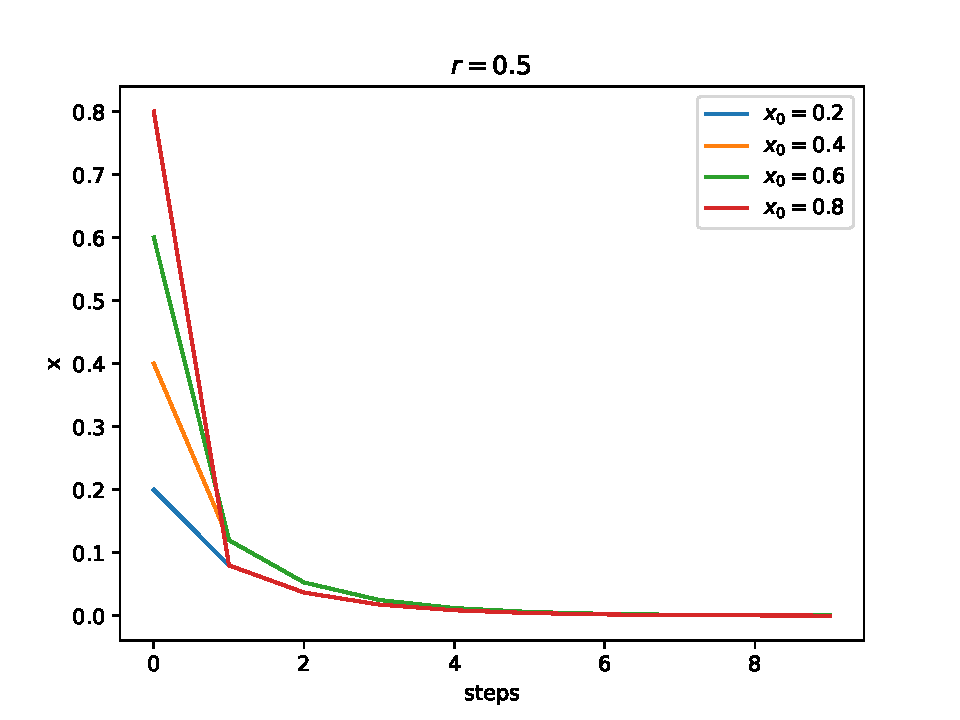
\includegraphics[scale=0.5]{1_0.pdf} & 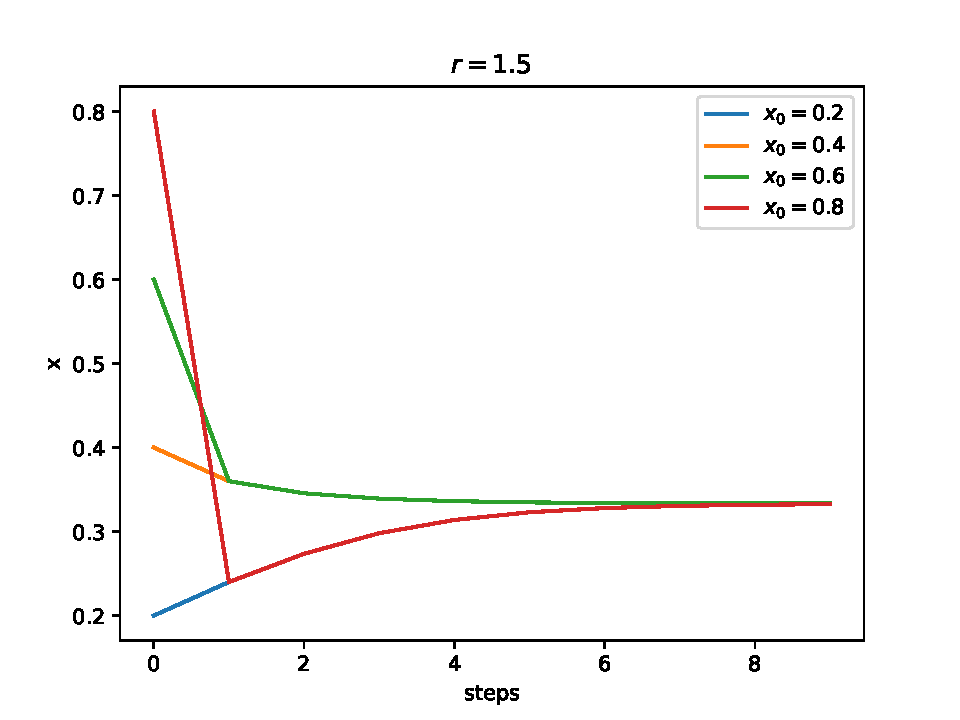
\includegraphics[scale=0.5]{1_1.pdf}
        \end{tabular}
        \centering
        \caption{选取$r = 0.5,\,r = 1.5$与不同初始值时迭代序列随步数的演化}
        \label{problem 1}
    \end{table}
    \par 
    可以看出在$r=0.5,\,r=1.5$这两个参数下, 对于不同的$x\in[0, 1]$, 序列均会收敛到稳定值, 
    对于两个不同的参数收敛值不同. 同时从图\ref{problem 1}的第二张图可以看出, 
    对于$r=1.5$, 不同初值$x_0$有着不单调的收敛行为. 

    \paragraph{2.}显然, 对于不同的$r$值, $x_n$将迅速收敛于某一特定的$x^*$初, 而
    与初值无关. $x^*$必将满足自洽方程: $x^* = f(x^*)$. 作为一个二元一次方程, 其存在两个根. 
    试判断并证明哪一个根才是最终收敛的不动点, 画出$x^*$随$r$的变化关系图. 
    一般而言, 其收敛阶$p$与收敛率$C$各是多少. 
    \paragraph{解: }
    自洽方程的根容易直接给出: $x^{*}_1 = 0,\,x^*_2 = 1-1/r$; 由不动点迭代的理论可知, 
    不动点稳定的判据是$|f'(x^*)| < 1$, $f'(x) = r - 2rx$, $x=0$为稳定点的条件是$0 < r < 1$, 
    $x = 1 - 1/ r$为稳定点的条件是$1 < r < 3$, 当$r > 3$时两个自洽方程的解均不是稳定点. 这与上一问
    的数值结果相符合. 将上述讨论绘制成图: 
    \begin{figure}[htbp]
        \centering
        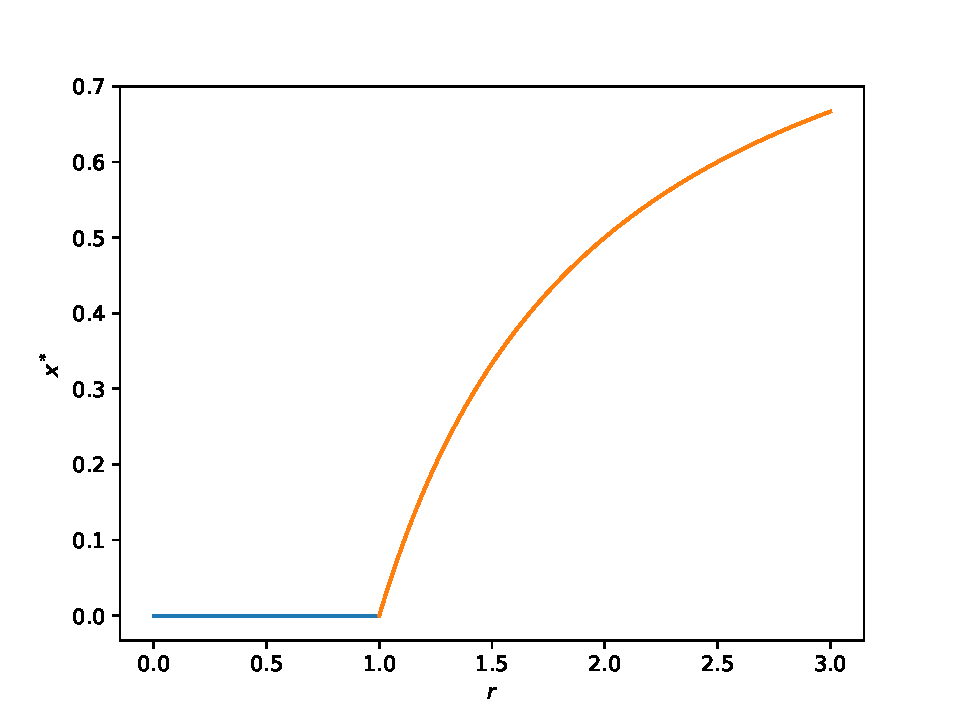
\includegraphics[scale=0.5]{2.pdf}
        \caption{收敛的不动点$x^*$随参数$r$的变化关系}
        \label{problem 2}
    \end{figure} 
    由不动点迭代的知识可知:
    \begin{equation}
        \frac{\epsilon_{n+1}}{\epsilon_n}\approx f'(x)
    \end{equation}
    那么对于本题中的情况, 只要导数不为零均对应着线性收敛$p=1$(导数为0可能对应着高阶的收敛, 开平方算法
    就是一个具体的例子). 那么$0 < r < 1$时收敛率为$r$, $1 < r < 3$时收敛率为$|2 - r|$. 
    
    \paragraph{3.}
    当$r$大于某个特定值$r_1$时, 上述条件无法满足. 取$r = r_1 + 0.1$以及不同的初值$x_0$, 计算序列$\{x_n\}$
    . 绘图观察并描述他们的行为. 
    \paragraph{解: }
    从第二问的分析可知, 本题目中要求的$r = 3.1$, 经过测试, 只有$x_0\in[0, 1)$时序列才是有界的. 
    \begin{figure}[htbp]
        \centering
        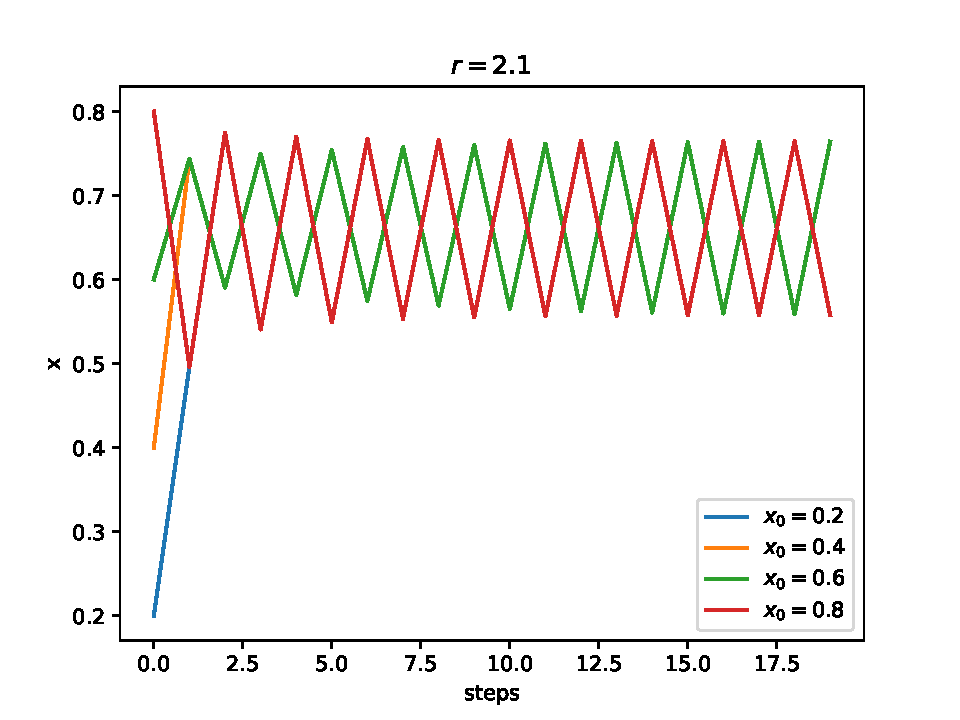
\includegraphics[scale=0.6]{3.pdf}
        \caption{$r=3.1$时不同初值下的序列随迭代步数的演化}
    \end{figure}

    \paragraph{4.}
    序列最终会在某两个特定值$x_1^*,\,x_2^*$之间震荡. 事实上, 考察复合迭代序列$x_{n+2} = f(f(x_n))$, 
    其定义的序列依旧收敛于某一个固定值, 从而依旧可以使用前述方法来分析. 试证明, 
    这类迭代收敛的必要条件是$|f'(x_1^*)f'(x_2^*)| \leq 1$, 并绘制出$x_1^*,\,x_2^*$随$r$的变化关系.
    \paragraph{解:}
    首先可以直接写出复合迭代的递推关系:
    \begin{equation}
        \begin{aligned}
            x_{n+2} &= f(f(x_n))\\
            & = rf(x_n)(1 - f(x_n))\\
            & = r^2(1 - x_n)(1 - rx_n(1 - x_n))
        \end{aligned}
    \end{equation}
    根据上式, 自洽方程可以写为:
    \begin{equation}
        x = r^2(1 - x_n)(1 - rx_n(1 - x_n))
    \end{equation}
    可以分解因式为:
    \begin{equation}
        0 = x(x - 1 + 1/r)(x^2 - (1 + 1/r)x + 1/r(1+1/r))
    \end{equation}
    容易给出自洽方程的四个根为:
    \begin{equation}
        \left\{
            \begin{aligned}
                x_1^* &= \frac{1}{2}\left(1 + \frac{1}{r} + \sqrt{1 - \frac{2}{r} - \frac{3}{r^2}}\right)\\
                x_2^* &= \frac{1}{2}\left(1 + \frac{1}{r} - \sqrt{1 - \frac{2}{r} - \frac{3}{r^2}}\right)\\
                x_3^* &= 1 - \frac{1}{r}\\
                x_4^* &= 0
            \end{aligned}
        \right.
    \end{equation}
    根据前几问的分析可知, 当$r > 3$时, 迭代序列不会稳定收敛到$x_3^*,\,x_4^*$, 那么对于复合迭代序列
    也不可能收敛到这两个值, 复合迭代序列一定收敛到前两个根. 从数值实验的结果可以断言(
    事实上这个结论可以直接计算验证):
    \begin{equation}
        \begin{aligned}
            f(x_1^*) &= x_2^*\\
            f(x_2^*) &= x_1^*
        \end{aligned}
    \end{equation}
    有了前面的结论之后可以分析复合迭代序列的稳定性, 在$x_1^*$附近$[f(fx_1^*)]' = f'(f(x_1^*))f'(x_1^*) = f'(x_2^*)f'(x_1^*)$, 
    有了这样的求导关系, 结合不动点的稳定性判据$|f'(x)| \leq 1$, 可以直接得到题目中的结论$|f'(x_1^*)f'(x_2^*)| \leq 1$.
    \par 
    下面绘制收敛点$x_1^*,\,x_2^*$随$r$的变化关系示意图, 可以从数值实验和理论计算两个角度来考虑. 
    理论分析已经在上文中给出, 现在考虑数值实验的具体方案, $r\in[3.1, 5.1]$, 从中选取100个点, 
    每个$r$均选取相同的初值$x_0 = 0.5$, 演化总步数为1000步(根据前几问的经验, 这么多步数应该足以收敛),
    取最后128个点作为收敛的点, 将这些点绘制成散点图, 并将理论计算的结果同时绘制作为对比: 
    \begin{figure}[htbp]
        \centering
        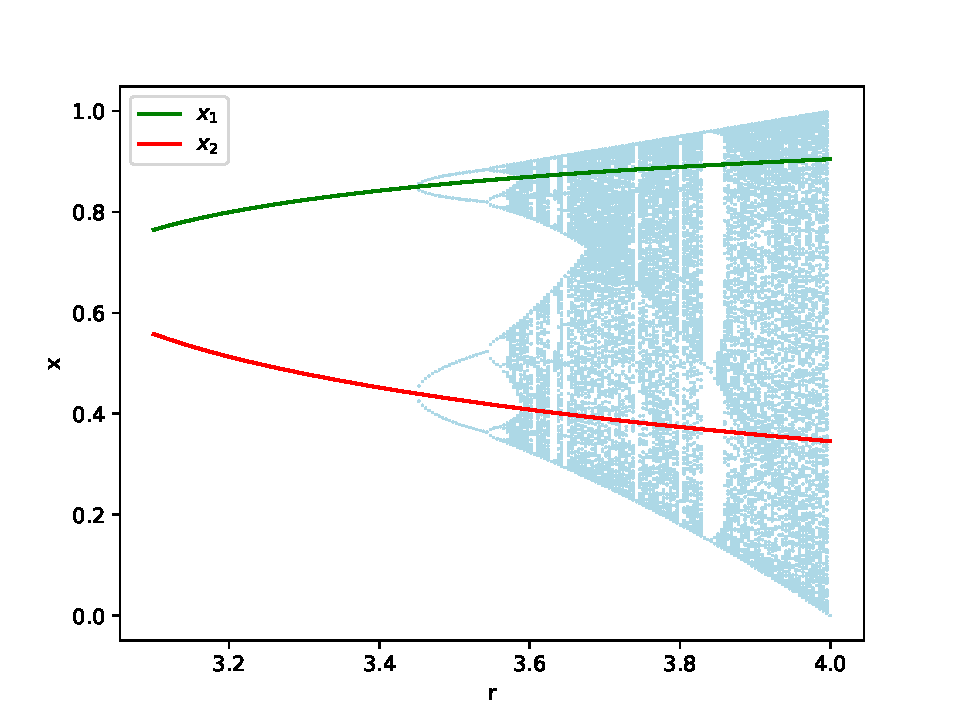
\includegraphics[scale=0.5]{4_1.pdf}
        \caption{$x_1^*,\,x_2^*$随$r$的变化关系}
    \end{figure}
    \par 
    从上图对比看出, 理论计算的结果在一定的范围内是有效的, 同时观察到了随着参数$r$的增长, 这一问理论分析的结果
    会变失效, 序列不在会只在两个点之间震荡, 收敛的结果会出现分岔现象.

    \paragraph{5.}
    继续缓慢增大$r$, 请展示周期为2的震荡逐渐变成周期4, 周期8……试定义一个量, 可以一般性描述序列向各类稳定
    震荡的平均收敛速度, 并可以由一段有限序列近似算出. 在$r\in(0, 4)$上等距取点, 绘制收敛速度随$r$的变化, 
    描述其与不同振荡周期的关系. 
    \paragraph{解:}
    选取$r\in[3.1, 3.58]$, 绘制绘制出稳定震荡点随$r$的变化关系如下图所示:
    \begin{figure}[htbp]
        \centering
        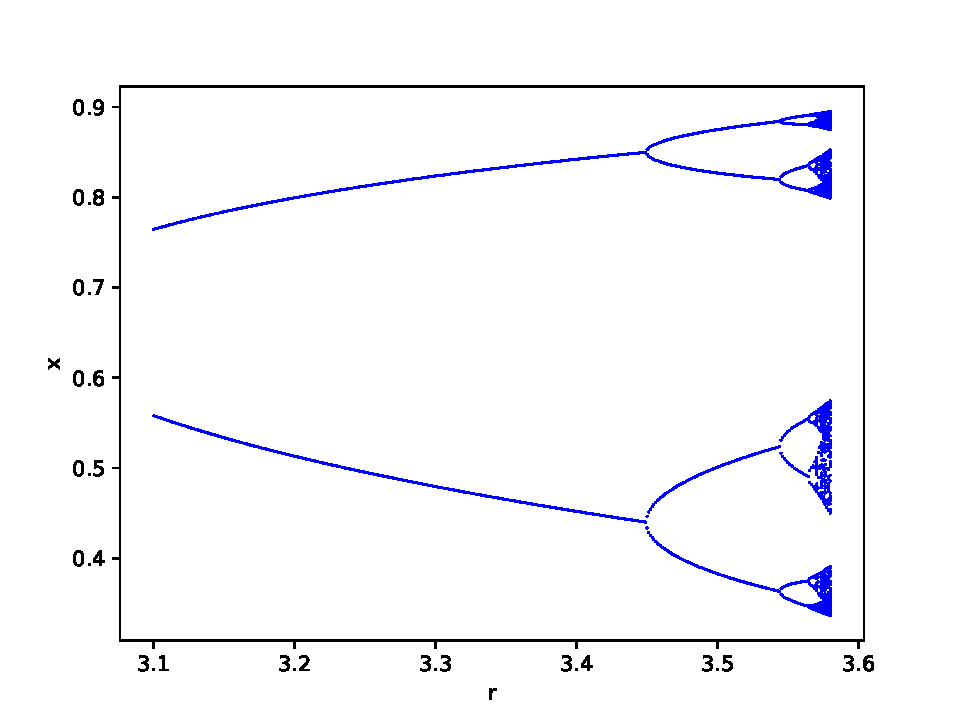
\includegraphics[scale=0.5]{5_1.pdf}
        \caption{不同$r$值时迭代序列的稳定震荡趋势}
    \end{figure}
    \par 
    下面给出采用$x_0\in[0.1,0.9]$均匀采点作为初值, $r=3.4,3.5,3.56,3.367$作为参数时迭代方程的演化:
    \begin{table}[htbp]
        \centering 
        \begin{tabular}[htbp]{cc}
            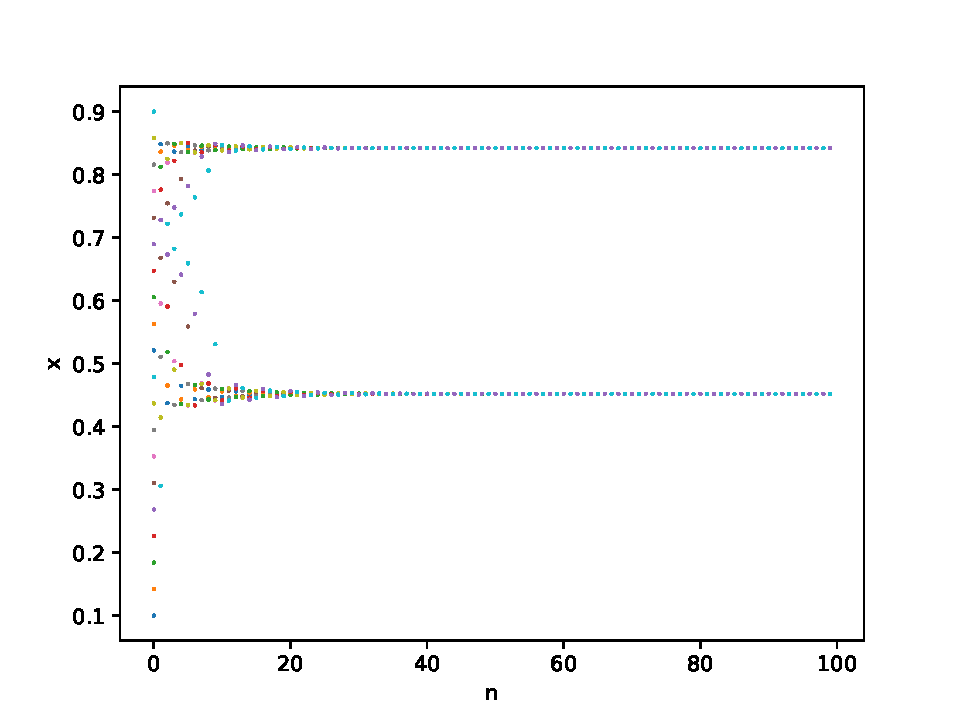
\includegraphics[scale=0.35]{5_2.pdf} & 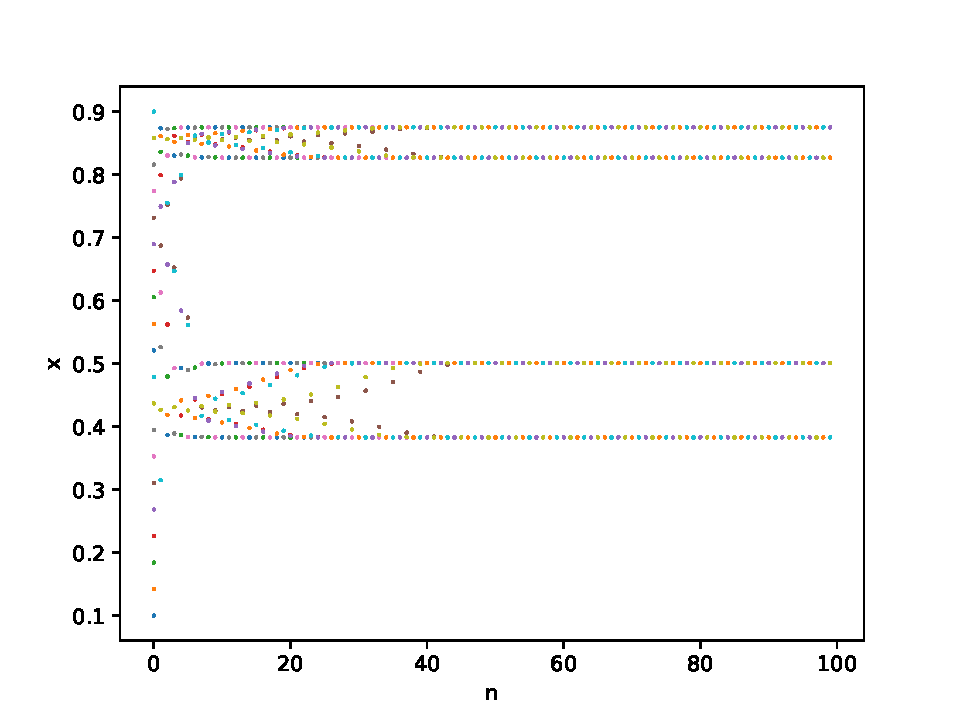
\includegraphics[scale=0.35]{5_4.pdf}\\
            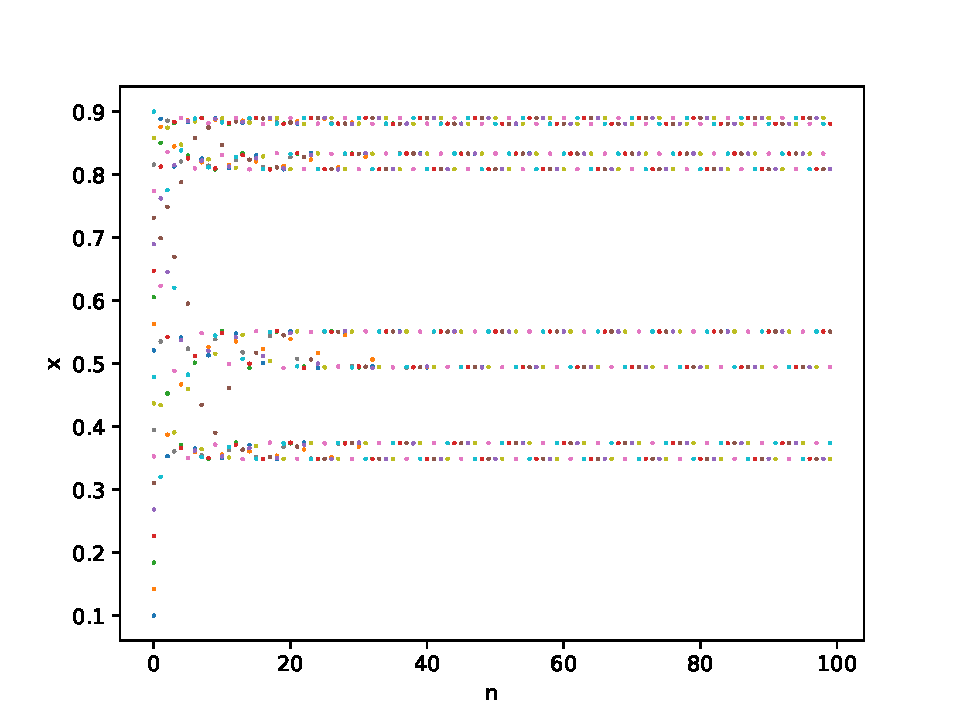
\includegraphics[scale=0.35]{5_8.pdf} & 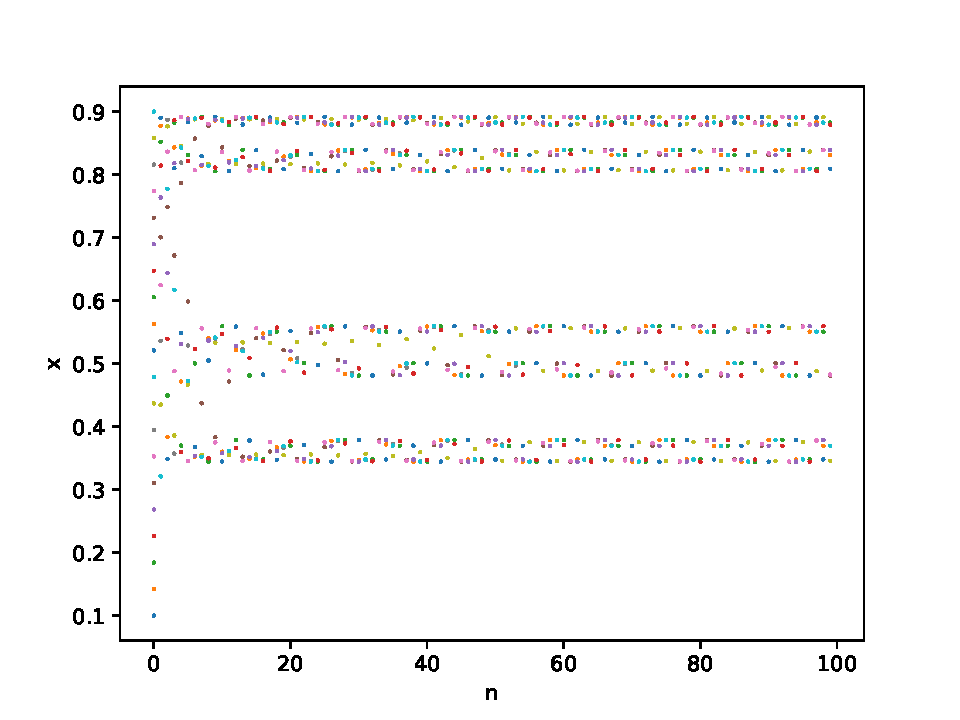
\includegraphics[scale=0.35]{5_16.pdf}\\
            \centering
        \end{tabular}
        \caption{采用不同的参数$r$值和不同的初始条件下的收敛结果}
    \end{table}
    \par 
    为了定义一个描述向稳定震荡收敛速度的量, 首先考虑怎样描述序列收敛到稳定震荡这样一件事情。我个人的想法是借用
    统计物理中系综的概念, 考虑在0时刻给定系统的初始值分布为$[0, 1]$上的平均分布(数值实现是可以在这个区间上
    等距均匀取点), 记为$\rho(x, 0)$, 在系统演化的过程中密度分布也会随时间演化, 记$n$时刻时系统的密度分布为
    $\rho(x, n)$. 如果系统在$n\to\infty$时可以达到稳定的震荡, \textbf{希望}密度函数$\rho(x, +\infty)$存在且可以表示为
    若干个$\delta$分布的和:
    \begin{equation}
        \rho(x, +\infty) = \frac{1}{N}\sum_{j=1}^{N}\delta(x - x_j)
    \end{equation}
    其中$x_j$是稳定震荡时能取到的一个值. 这样的分布任意阶矩都存在,可以完全由任意阶矩$M_j := \int\rho(x)x^j\d x$
    来描述, 为了方便起见, 这里考虑用平均值来描述, 首先绘制出不同$r,n$时平均值$\braket{x}$的变化关系, 考察一下这种
    描述方式到底现不现实, 经过数值实验后发现, 完全不太现实, 事实上密度函数并不收敛, 也是震荡的. 
    \par
    为了描述收敛, 考虑定义另外的序列$y_n$(原序列的切萨罗和):
    \begin{equation}
        y_n := \frac{\sum_{j = 1}^{n}x_j}{n}
    \end{equation}
    容易想象, 对于一个稳定震荡的序列$x_n$, 这样构造出的$y_n$应该是一个收敛的序列. 为了进一步确信, 
    考虑以周期2为例绘制出原序列$x_n$和切萨罗求和过后的序列$y_n$($x_0 = 0.5$):
    \begin{figure}[htbp]
        \centering
        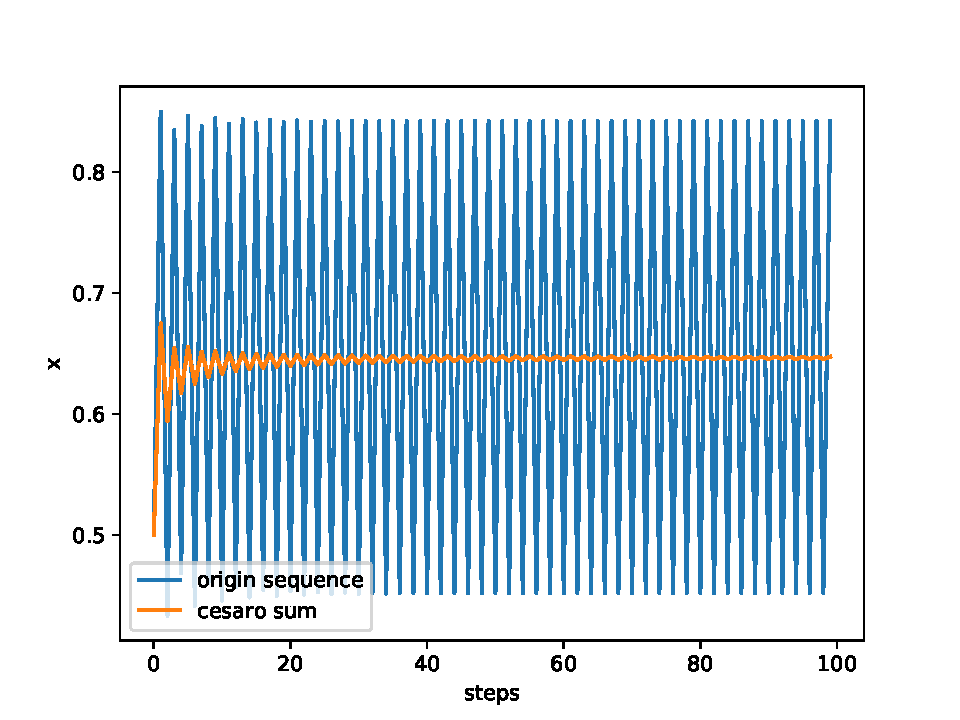
\includegraphics[scale=0.5]{6_cesaro_p=2.pdf}
        \caption{周期2时原序列与切萨罗求和之后的比较}
    \end{figure}
    \par 
    将不同周期的震荡序列的切萨罗和绘制在同一张图中比较($x_0 = 0.5$):
    \begin{figure}[htbp]
        \centering 
        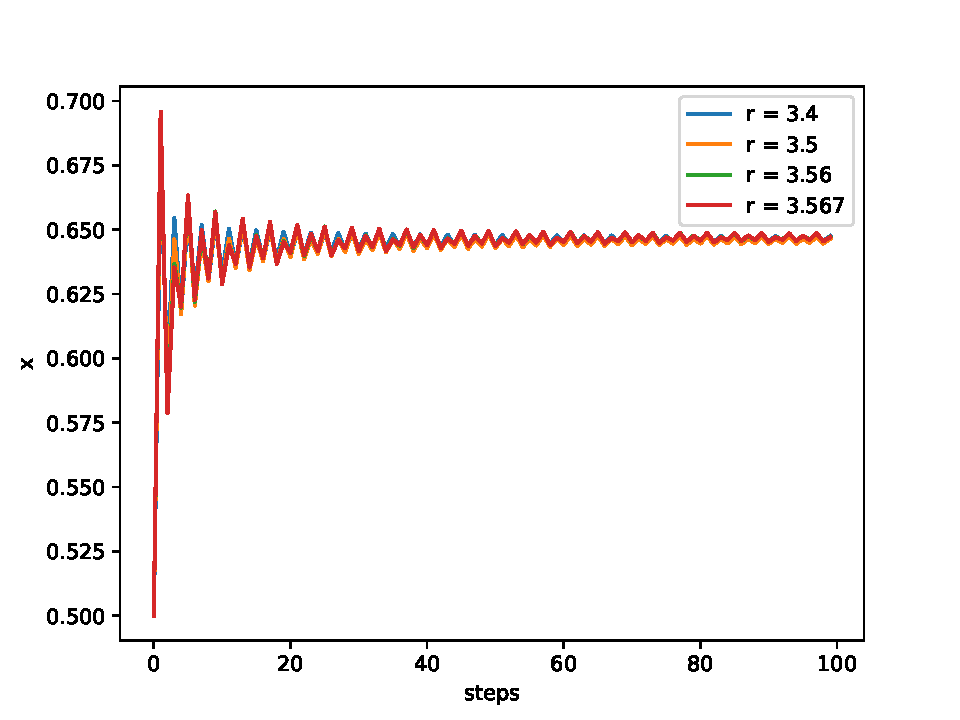
\includegraphics[scale=0.5]{6_cesaro_compare.pdf}
        \caption{不同震荡周期的序列的切萨罗和的收敛行为$x_0=0.5$}
    \end{figure}
    \par 
    从图中可以看出, 对于初值$x_0=0.5$不同周期的序列收敛速度基本一致, 尝试了其他的初值, 
    发现切萨罗和的收敛行为对初值敏感, 不适合作为一个描述收敛的量:
    \begin{figure}[htbp]
        \centering
        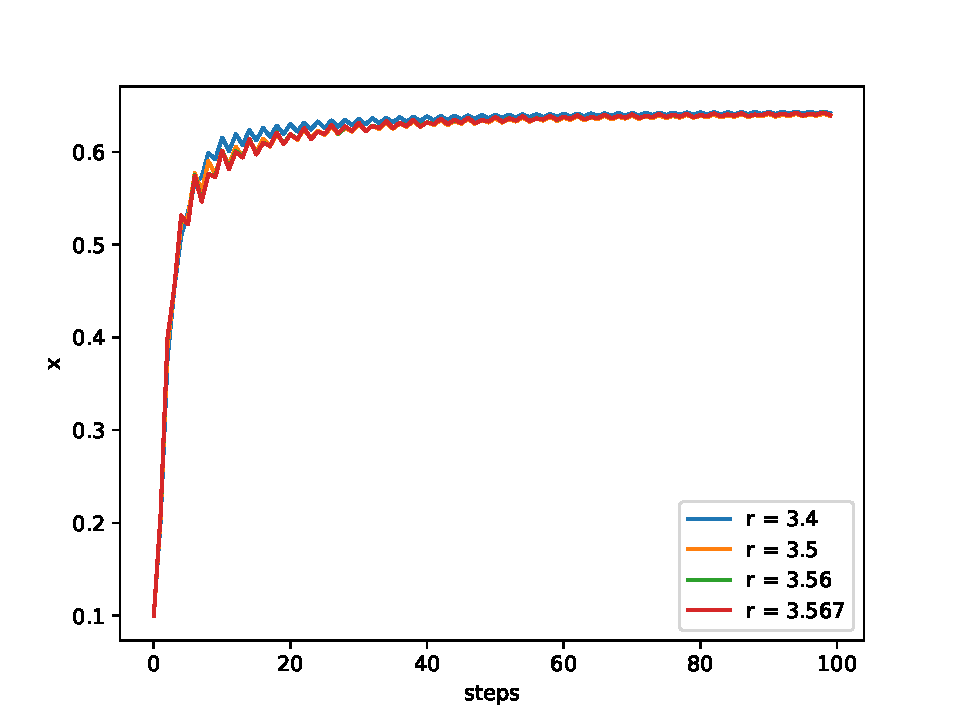
\includegraphics[scale=0.5]{6_cesaro_compare_another.pdf}
        \caption{不同震荡周期的序列的切萨罗和的收敛行为$x_0=0.1$}
    \end{figure}
    \paragraph{6.}
    绘制震荡值随$r$的变化关系. 依次缩小绘图范围, 将坐标原点分别放在周期1、周期2的分岔点, 周期2、周期4的
    分岔点, 周期4、周期8的分岔点, 描述你观察到的现象.
    \paragraph{解:}
    有了第5问中分岔随$r$变化的关系, 大致可以确定各个分岔的位置. 为了精确描述周期1与周期2的分岔点, 将$r$的值选取在
    在$[2.997,2.9992]$之间, 均匀取200个点, 以$x_0 = 0.5$为初始值, 演化5000步, 取最后64个点作为收敛的
    点绘制在图中:
    \begin{figure}[htbp]
        \centering
        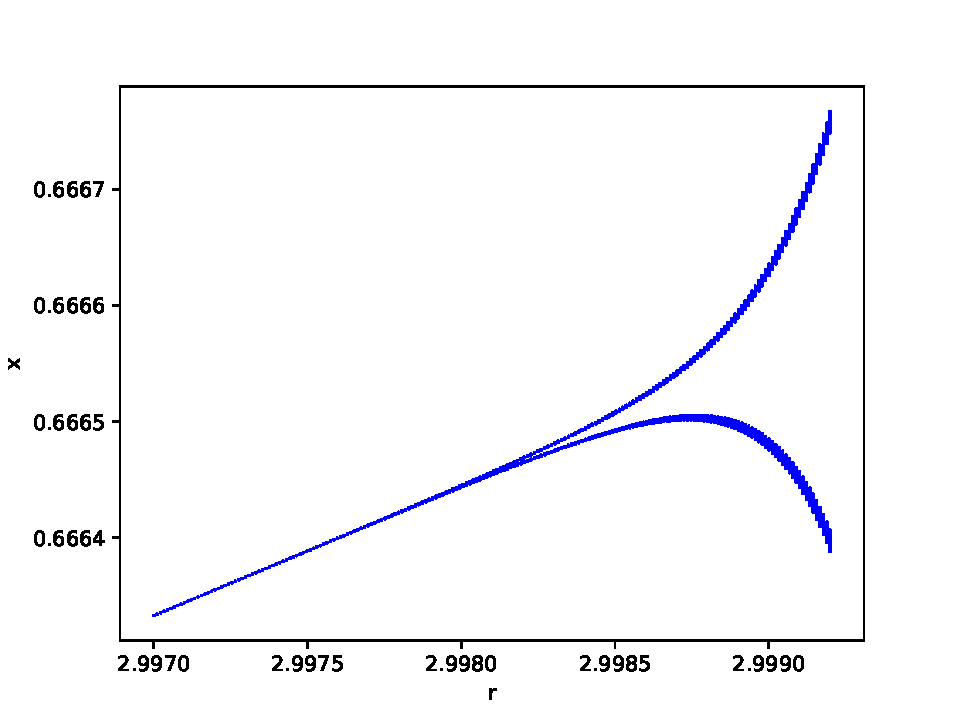
\includegraphics[scale=0.5]{6_1.pdf}
        \caption{周期1与周期2分岔点}
    \end{figure}
    \par 
    从图中可以看出, 周期一与周期二的分岔点$r\approx 2.9989$(精确到万分位), 这与前几问中的理论分析($r=3$)略有差别, 个人认为是数值精度造成的.
    \par 
    为了精确描述周期2与周期4的分岔点, $r$选取在$[3.448, 3.4505]$之间, 均匀取200个点, 以$x_0 = 0.5$为初始值,
    演化5000步, 取最后64个点作为收敛的点绘制在图中:
    \begin{figure}[htbp]
        \centering
        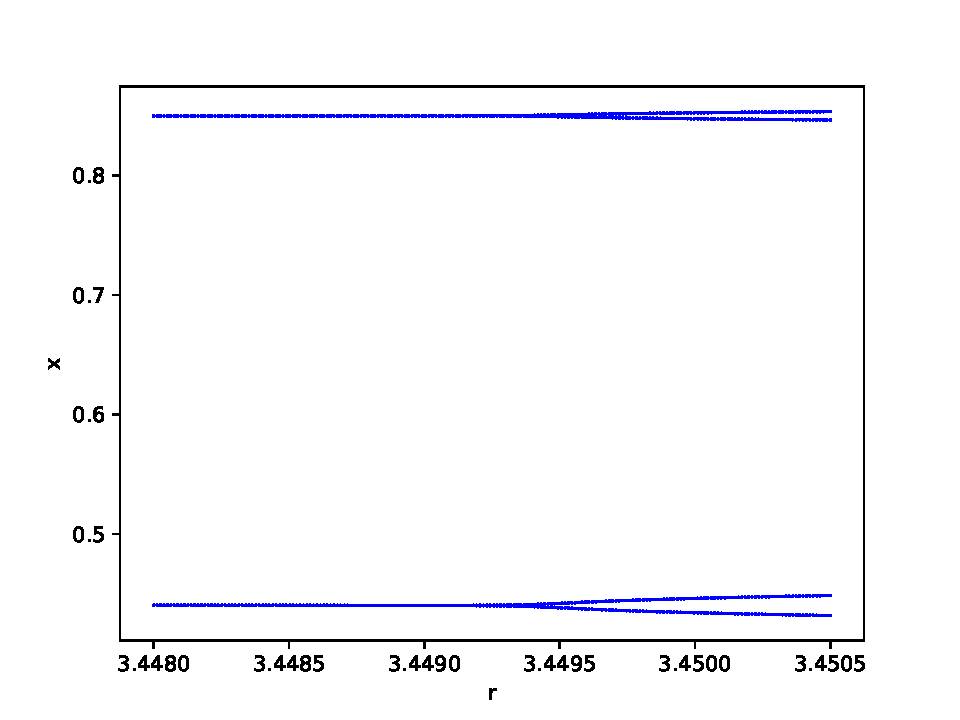
\includegraphics[scale=0.5]{6_2.pdf}
        \caption{周期2与周期4的分岔点}
    \end{figure}
    \par 
    从图中可以看出, 周期2与周期4的分岔点$r\approx 3.4490$(精确到万分位).
    \par 
    为了精确描述周期4与周期8的分岔点, $r$选取在$[3.54, 3.55]$之间, 均匀取点200个, 以$x_0=0.5$为初始值, 
    演化10000步, 取最后128个点作为收敛的点绘制在图中:
    \begin{figure}[htbp]
        \centering
        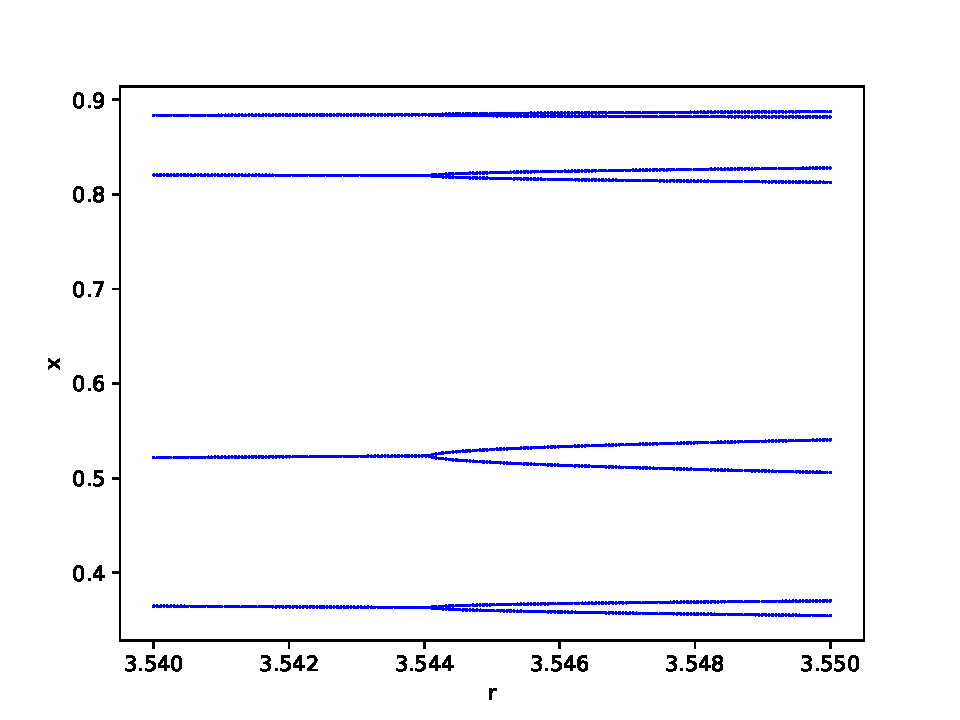
\includegraphics[scale=0.5]{6_3.pdf}
        \caption{周期4与周期8的分岔点}
    \end{figure}
    \par 
    从图中可以看出, 周期4和周期8的分岔点$r\approx 3.5440$(精确到万分位)
    \par 
    为了精确描述周期8与周期16的分岔点, $r$选取在$[3.562, 3.568]$之间, 均匀取点300个, 以$x_0 = 0.5$为初始值
    演化10000步, 取最后128个点作为收敛的点绘制在图中:
    \begin{figure}[htbp]
        \centering
        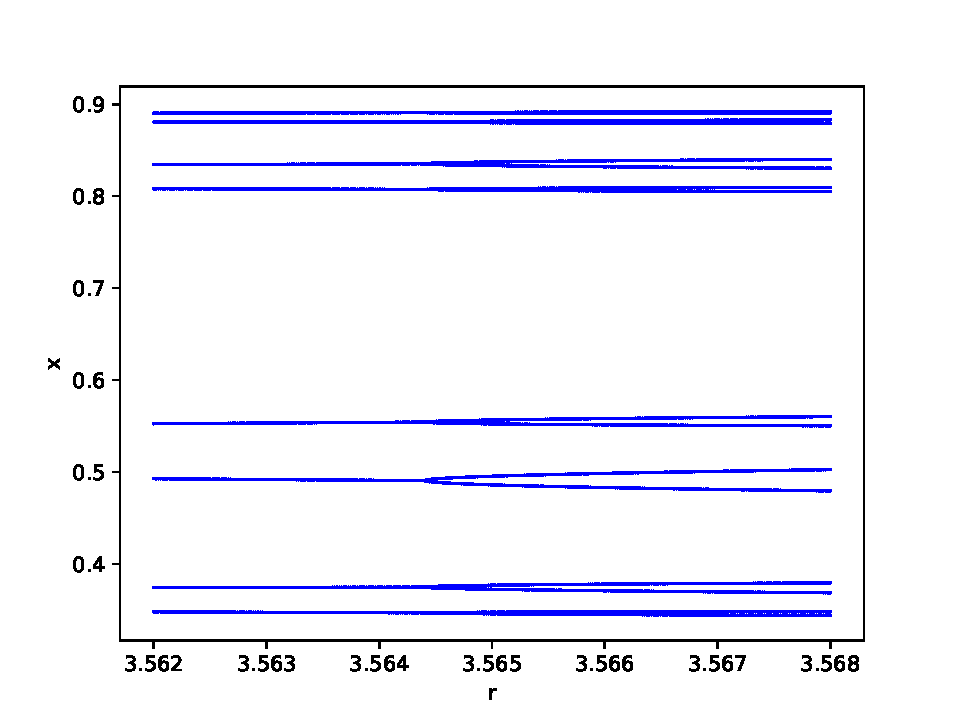
\includegraphics[scale=0.5]{6_4.pdf}
        \caption{周期8与周期16的分岔点}
    \end{figure}
    \par 
    从图中可以看出, 周期8与周期16的分岔点$r\approx 3.5644$(精确到万分位)
    \par 
    为了进一步分析分岔现象, 将$r$选取在$[3.5686, 3.5689]$, 均匀取点300个, 以$x_0 = 0.5$为初始值, 演化10000步, 
    取最后256个点作为收敛的点绘制在图中: 
    \begin{figure}[htbp]
        \centering
        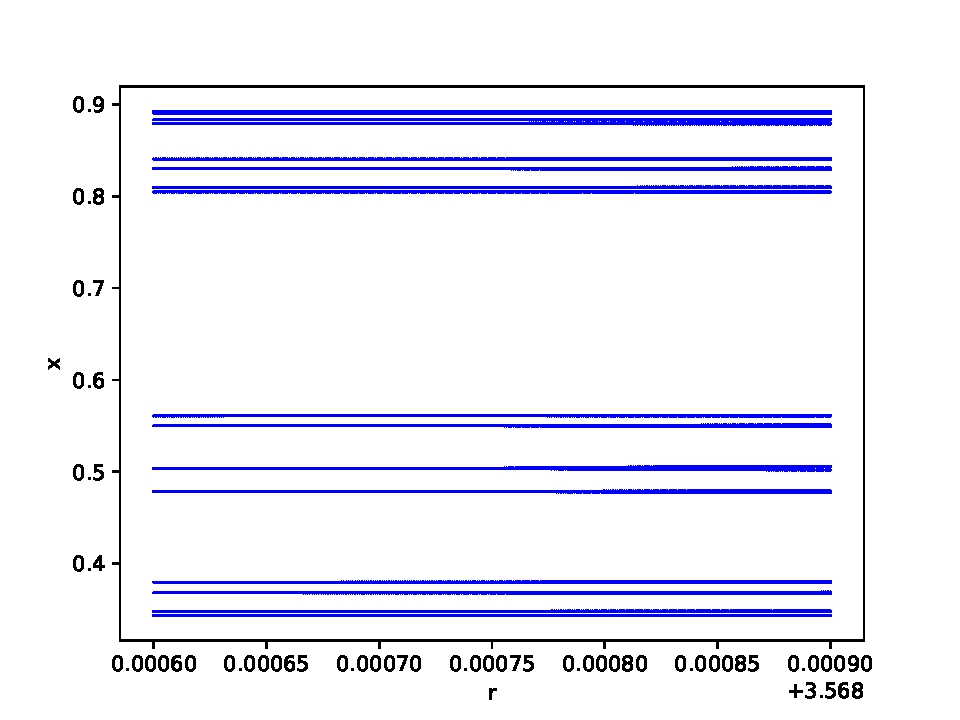
\includegraphics[scale=0.5]{6_5.pdf}
        \caption{周期16到周期32的分岔点}
    \end{figure}
    从图中可以得到, 周期16到周期32的分岔点处$r = 3.56874$

    \paragraph{7.}
    计算相邻分岔点之间的横轴距离$\Delta r$, 说明相邻$\Delta r$之比渐进于一个常数$F$, 计算出$F$与
    无穷周期分岔点$r_{\infty}$的值.
    \paragraph{解:}
    有了第6问的数据, 可以直接计算出:
    \begin{equation}
        \left\{
        \begin{aligned}
            \Delta r_{1} &= 3.4490 - 2.9980 = 0.4510\\
            \Delta r_{2} &= 3.5440 - 3.4490 = 0.0950\\
            \Delta r_{3} &= 3.5644 - 3.5440 = 0.0204\\
            \Delta r_{4} &= 3.56874 - 3.5644 = 0.00430\\
        \end{aligned}
        \right.
    \end{equation}
    那么可以计算出相邻$\Delta r$的比值:
    \begin{equation}
        \left\{
        \begin{aligned}
            F_1 = 0.211\\
            F_2 = 0.215 \\
            F_3 = 0.211 \\
        \end{aligned}
        \right.
    \end{equation}
    那么可以将$F$取为$F=0.211$, 无穷周期分岔点$r$可以按下式计算:
    \begin{equation}
        r_\infty = r_{8\rightarrow 16} + \Delta r_{4}\cdot\sum_{j=0}^{+\infty}F^j = 3.5712
    \end{equation}
    为了验证这一点, 将$r$选取在$[3.562, 3.629]$, 均匀取点400个, 以$x_0 = 0.5$为初始值, 演化10000步将最后
    512步作为收敛点绘制在图中:
    \begin{figure}[htbp]
        \centering
        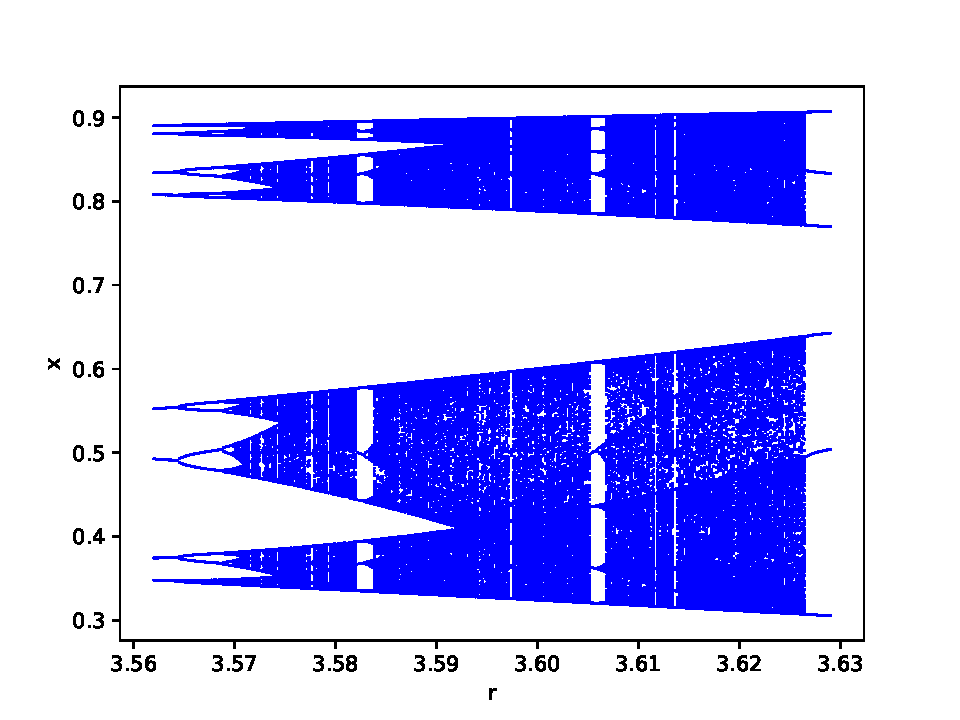
\includegraphics[scale=0.5]{6_another.pdf}
        \caption{分岔现象的大致图像}
    \end{figure}
    可以看到第一次出现无穷周期的$r$值就应该在3.57附近, 但是显然收敛值随$r$的变化显示出了异常复杂的图样, 
    在图中可以看到从有周期到无周期再到有周期的变化, 也能在其中看到奇怪的颜色较深的曲线, 这表明收敛点更倾向于
    集中在这些地方.

    \paragraph{8.}
    对于$r=4$的情形, 试解析求解该迭代序列, 论证此时一般不存在稳定的的振荡周期.
    \paragraph{解: }
    做变换$x = \sin^2(y)$, $x$的取值范围为$[0, 1]$, 那么$y$的取值范围为$[0, \pi/2]$, 在这个
    范围内$x\leftrightarrow y$之间的变换为一一映射. 容易将迭代关系写为:
    \begin{equation}
        \begin{split}
            \sin^2(y_{n+1}) &= x_{n+1} = r(1 - x_n)x_n\\
            & = r\cos^2(y_n)\sin^2(y_n)\\
            & = \frac{r}{4}\sin^2(2y_n)
        \end{split}
    \end{equation}
    如果取$r = 4$, 那么可以得到$\sin^2(y_{n+1}) = \sin^2(2y_n)$, 由于我们限制了$y$的取值范围, 
    因此得到$y_{n+1}$与$y_n$的关系:
    \begin{equation}
        y_{n+1} = 
        \left\{
        \begin{aligned}
            &2y_n\quad\quad \text{if}\,\, 2y_n < \pi/2\\
            &2y_n - \pi \quad\quad \text{if}\,\,\pi / 2 \leq 2y_n \leq \pi 
        \end{aligned}
        \right.
    \end{equation}
    那么$y_n$总可以表示为: $y_n = 2^n y_0 - N\pi$, 其中$N$为一个正整数. 
    那么:
    \begin{equation}
        x_n = \sin^2{y_n} = \sin^2(2^ny_0)
    \end{equation}
    若想要$x_n$呈现出周期性, 那么$2^ny_0$至少要满足$2^ny_0 / \pi$的小数部分只有有限种
    状态, 比如对应$y_0$是$\pi$有理数倍的情况, 对于无理数的情况, 我无法证明小数点后面的数值
    只取有限个状态(但是感觉上是不对的), 这种初值对应的序列不可能存在稳定的振荡周期.

    \paragraph{9.}
    选择另一个你喜欢的函数$g(x)$, 其在从原点开始的某段区域上是凸函数, 将$x(1-x)$替换成为$g(X)$,
    重复1-7问的计算, 说明可以看到类似的现象, 并得到完全相同的$F$值. 
    \paragraph{解:}
    将函数选为: $g(x) = 2 - \cosh(x)$, 它是一个$[0,1]$之间的凸函数, 递推关系可以写为:
    \begin{equation}
        x_{n+1} = r(2 - \cosh(x))
    \end{equation}
    自洽方程的根并不能解析算出. 
    \subparagraph{9-1:}
    首先令$r=0.5,r=1.5$绘制出迭代序列
    \begin{table}[htbp]
        \centering
        \begin{tabular}[htbp]{cc}
            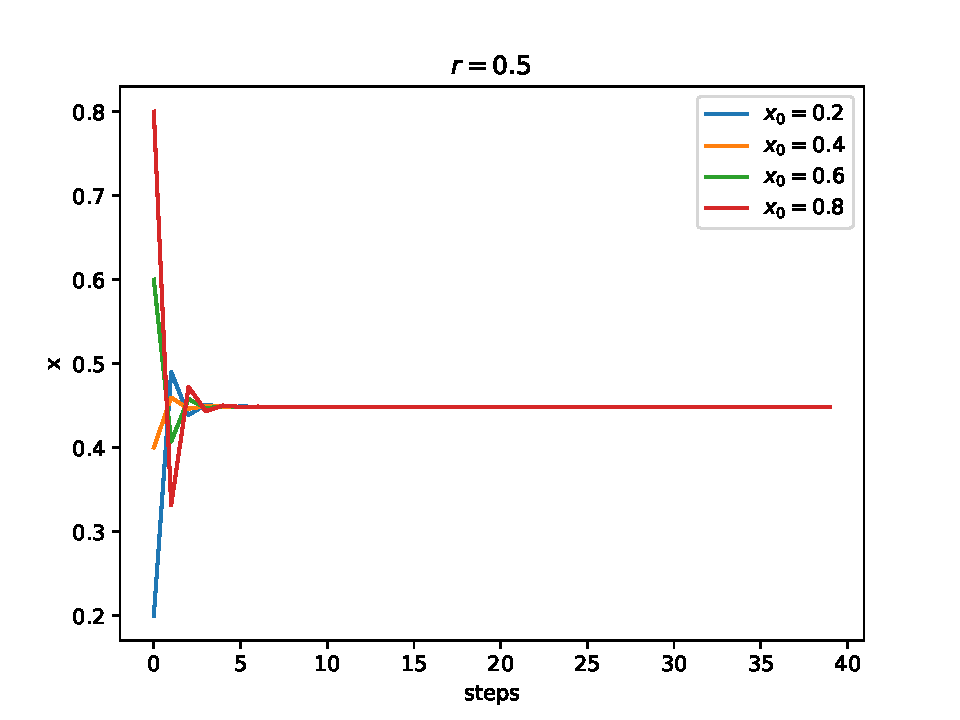
\includegraphics[scale=0.35]{9_1_0.pdf} & 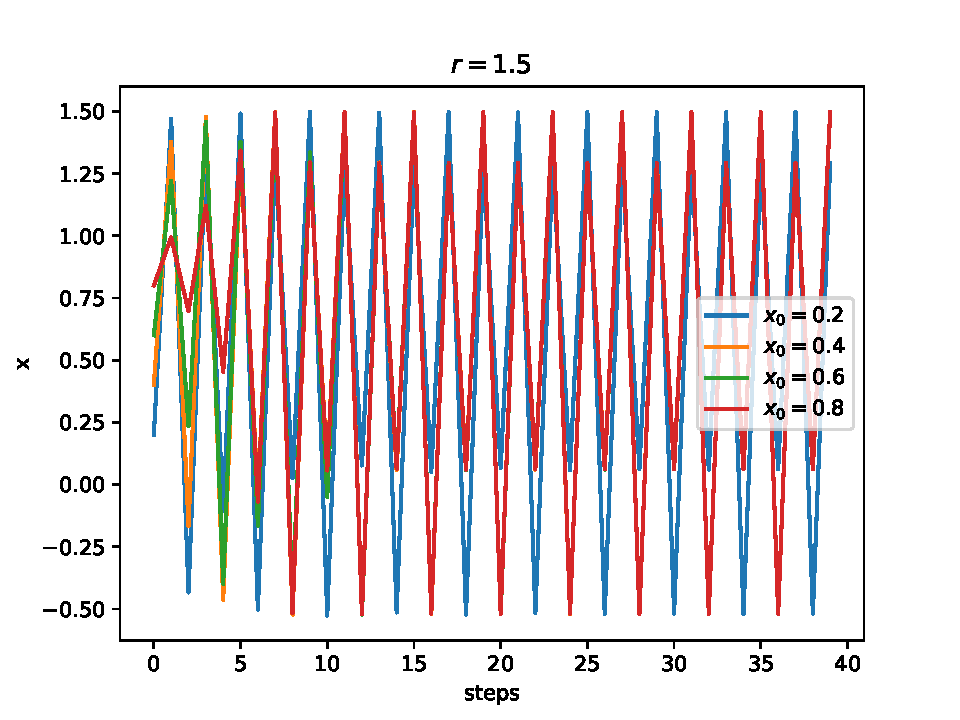
\includegraphics[scale=0.35]{9_1_1.pdf}\\
        \end{tabular}
        \caption{$r=0.5,\,1.5$时迭代序列收敛的情况}
    \end{table}
    可以看出$r=0.5$时迭代序列收敛, 但是$r=1.5$时迭代序列产生了震荡.
    \subparagraph{9-2:}
    由于自洽方程的根难以解析求解, 考虑直接绘制出收敛点随$r$的变化关系, 同时在其中观察分岔现象.
    $r$在区间$[0.1, 1.75]$中等距选点200个, 选取初始值$x_0=0.5$, 演化5000步, 取最后256个点作为收敛的点绘制在图中. 
    \begin{figure}[htbp]
        \centering
        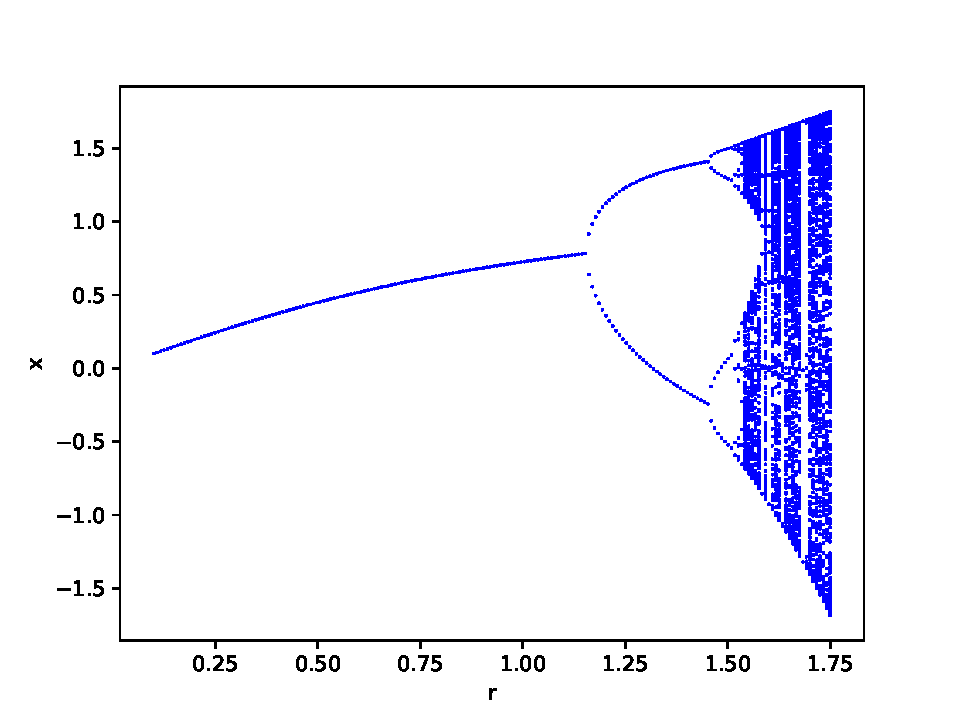
\includegraphics[scale=0.5]{9_2.pdf}
        \caption{收敛点随$r$的变化与分岔现象}
    \end{figure}
    \subparagraph{9-3:}
    现在来探究分岔点具体的位置.(原题目中有些解析计算的问题本例中无法重复)
    首先给出周期1到周期2分岔点的示意图, $r$在区间$[1.152,1.158]$中均匀取点400个, 初值为$x_0 = 0.5$, 演化5000步
    取最后64个点作为收敛的点,
    \begin{figure}[htbp]
        \centering
        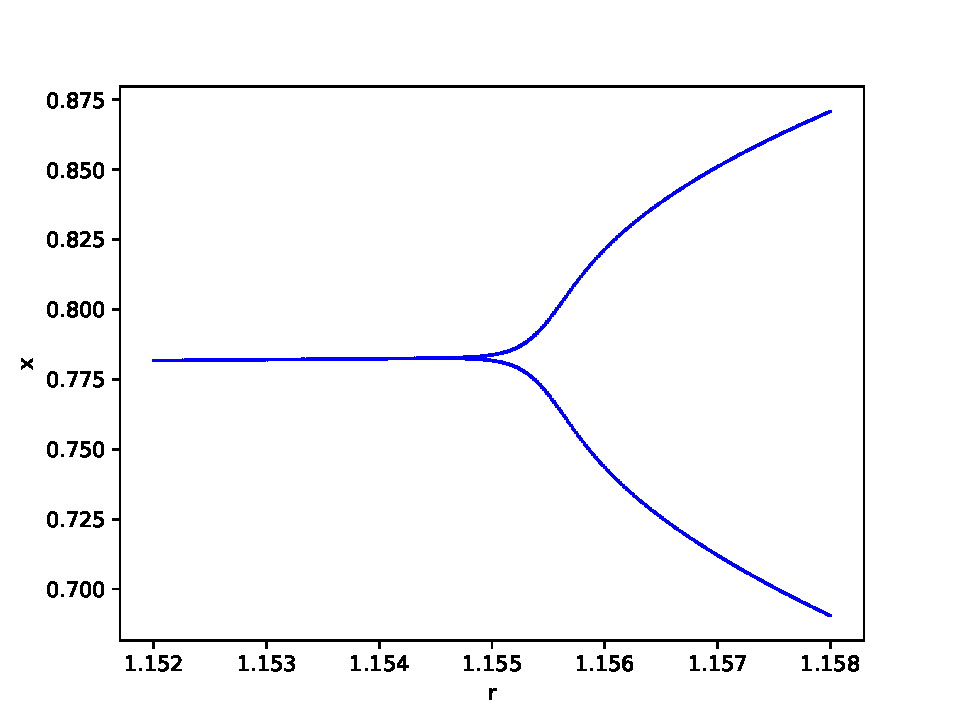
\includegraphics[scale=0.5]{9_3_1.pdf}
        \caption{周期1与周期2分岔点附近示意图}
    \end{figure}
    \par 
    分岔点的位置$r \approx 1.1547$
    \par 
    做出周期2到周期4分岔的示意图, $r$在区间$[1.450,1.455]$中均匀取点400个, 初值为$x_0 = 0.5$, 演化5000步
    取最后64个点作为收敛的点,
    \begin{figure}[htbp]
        \centering
        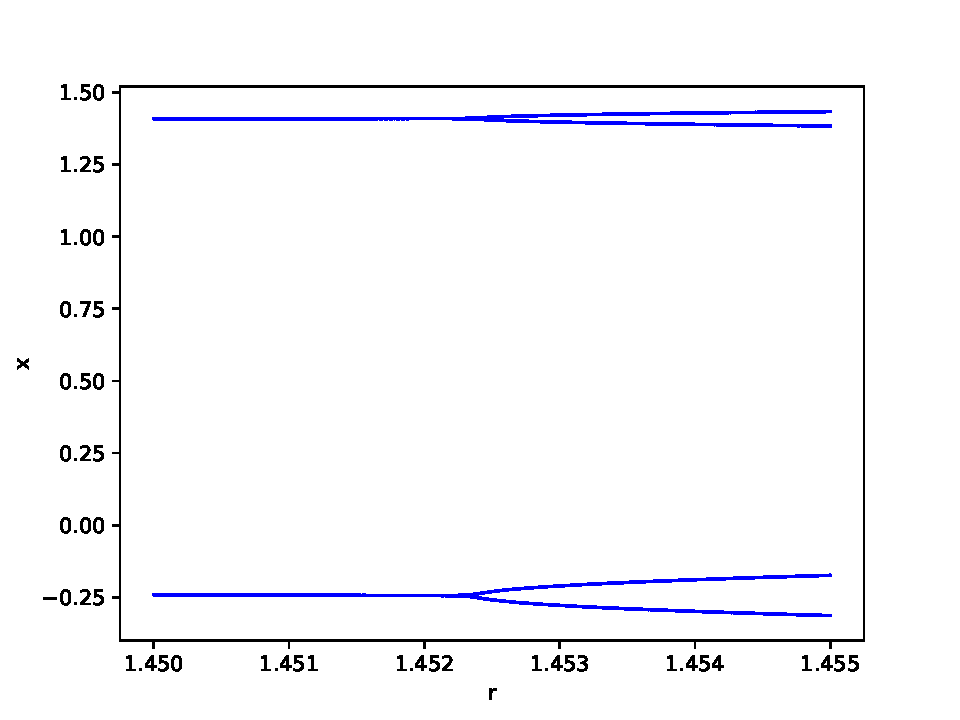
\includegraphics[scale=0.5]{9_3_2.pdf}
        \caption{周期2与周期4分岔点附近示意图}
    \end{figure}
    \par 
    分岔点的位置$r \approx 1.4522$

    \par 
    做出周期4到周期8分岔的示意图, $r$在区间$[1.50,1.52]$中均匀取点400个, 初值为$x_0 = 0.5$, 演化5000步
    取最后64个点作为收敛的点,
    \begin{figure}[htbp]
        \centering
        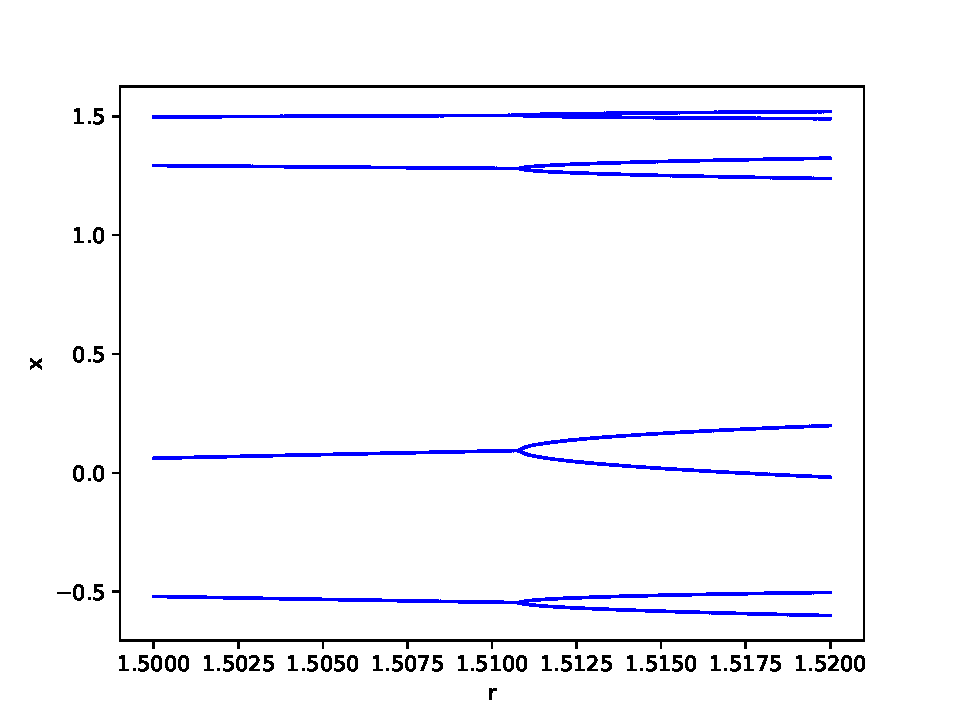
\includegraphics[scale=0.5]{9_3_3.pdf}
        \caption{周期4与周期8分岔点附近示意图}
    \end{figure}
    \par 
    分岔点的位置$r \approx 1.5107$

    \par 
    做出周期8到周期16分岔的示意图, $r$在区间$[1.52,1.526]$中均匀取点400个, 初值为$x_0 = 0.5$, 演化10000步
    取最后256个点作为收敛的点,
    \begin{figure}[htbp]
        \centering
        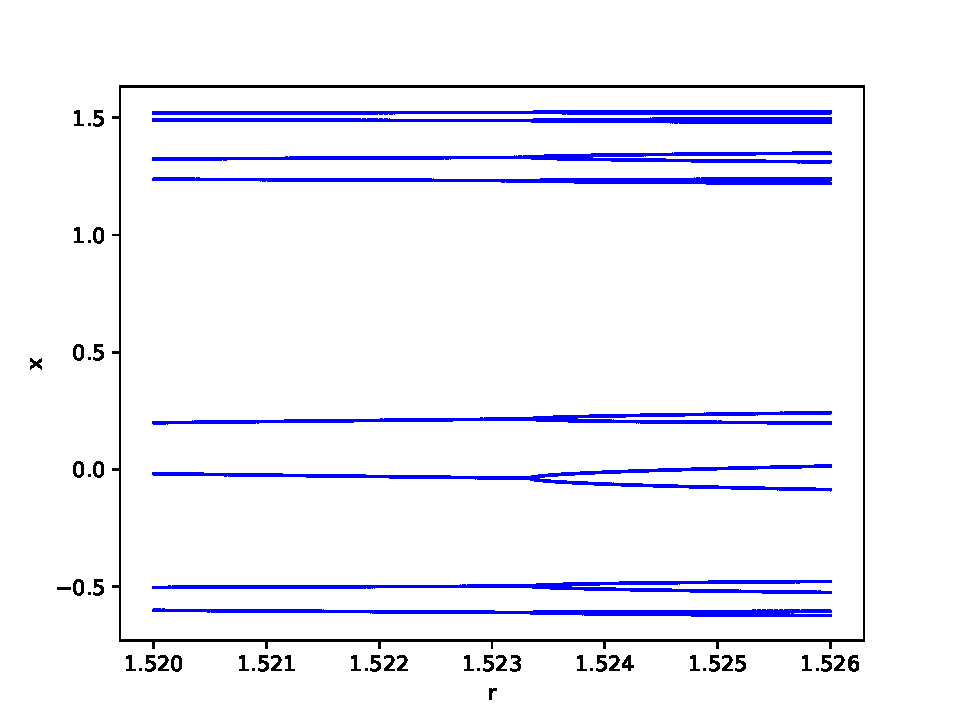
\includegraphics[scale=0.5]{9_3_4.pdf}
        \caption{周期8与周期16分岔点附近示意图}
    \end{figure}
    \par 
    分岔点的位置$r \approx 1.5233$

    \par 
    做出周期16到周期32分岔的示意图, $r$在区间$[1.5259,1.5261]$中均匀取点400个, 初值为$x_0 = 0.5$, 演化10000步
    取最后256个点作为收敛的点,
    \begin{figure}[htbp]
        \centering
        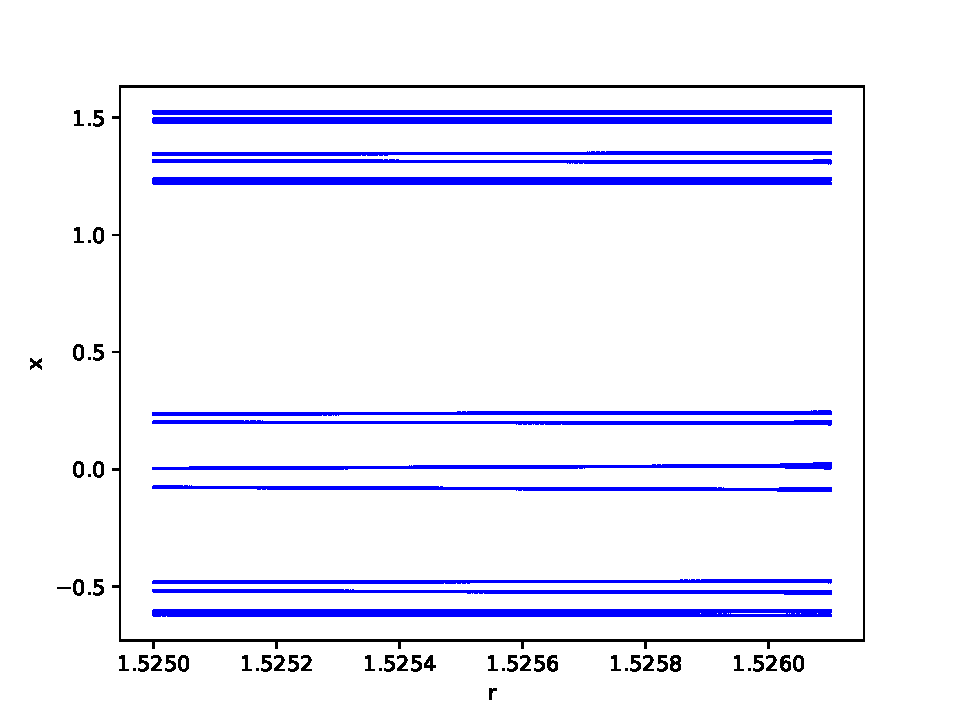
\includegraphics[scale=0.5]{9_3_5.pdf}
        \caption{周期16与周期32分岔点附近示意图}
    \end{figure}
    \par 
    分岔点的位置$r \approx 1.5260$
    \par 为了直观起见给出分岔的总览,
    \begin{figure}
        \centering
        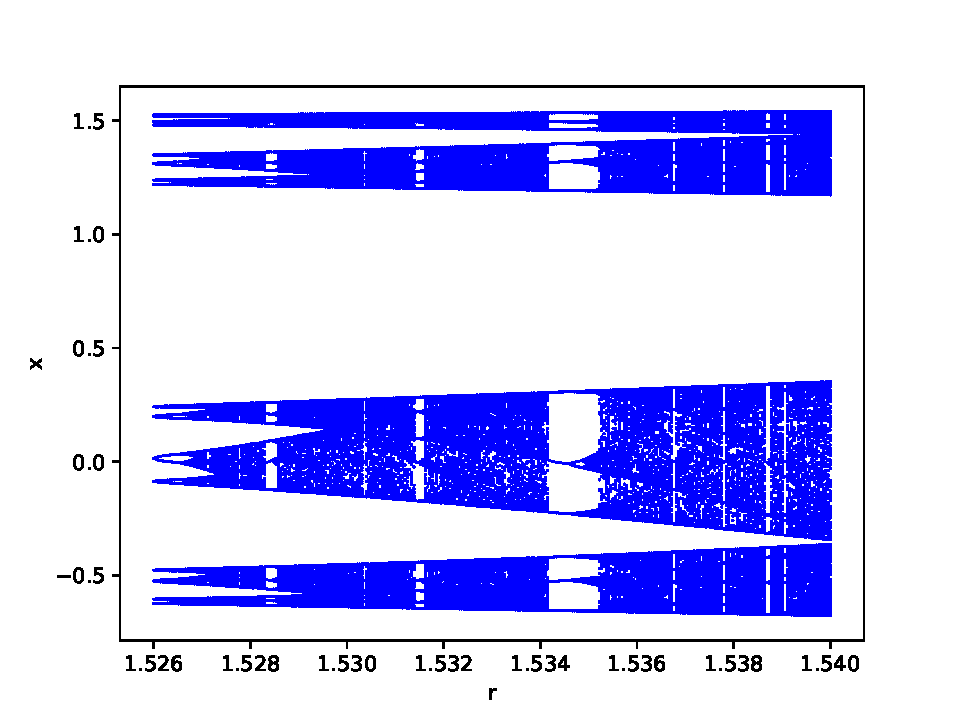
\includegraphics[scale=0.5]{9_3_another.pdf}
    \end{figure}
    \par 
    有了这些数据后可以直接算出相邻分岔点之间的距离:
    \begin{equation}
        \left\{
        \begin{aligned}
            \Delta r_1 &= 0.2975 \\
            \Delta r_2 &= 0.0585 \\
            \Delta r_3 &= 0.0126 \\
            \Delta r_4 &= 0.0027
        \end{aligned}
        \right.
    \end{equation}
    那么可以计算比值:
    \begin{equation}
        \left\{
        \begin{aligned}
            F_1 &= 0.197\\
            F_2 &= 0.216\\
            F_3 &= 0.222
        \end{aligned}
        \right.
    \end{equation}
    与之前的F对比可以看出, 两者基本相等.
\end{document}